\section{Auswertung}

Die in der Auswertung bestimmten Ausgleichsrechnungen werden mit
dem Python Paket \emph{scipy.optimize}\cite{scipy} durchgeführt.

\subsection{Fehlerrechnung}

Die für die Auswertung benötigt Mittelwerte werden mit

\begin{equation}
  \label{eq: mittel}
  \ov{x}=\frac{1}{N}\sum_i^N x_i
\end{equation}
berechnet. Die zugehörige Standartabweichung des Mittelwertes lautet:

\begin{equation}
  \label{eq: standartabweichung}
  \sigma_{\ov{x}}=\sqrt{ \frac{1}{N(N-1)} \sum_i^N (x_i-\ov{x})^2}.
\end{equation}

Weiterhin werden die Fehler mit der Gaußschenfehlerfortpflanzung fortgepflanzt:

\begin{equation}
  \label{eq: gauss_fehler}
  \sigma_f= \sqrt{ \sum_i^M \left(\frac{\partial f}{\partial x_i} \sigma_{x_i}\right)^2}.
\end{equation}

\subsection{Volumenbestimung}

Um die Saugvermögen der Drehschieber- bzw. Tubropumpe zu bestimmen, wird das Gesamtvolumend des Aufbaus benötigt.
Hierbei ist zu beachten das sich die Volumina vom Drehschieber- und Turboaufbau jeweils voneinander unterscheiden.
Als Messfehler wird $\SI{0.5}{\milli\meter}$ angenommen, außer beim Volumen des Tankes. Dort werden die
Bauteile mit einem Fehler von $\SI{2.5}{\milli\meter}$ behaftet. Der vergrößerte Fehler kommt dadurch zustande, dass die
Dicke des Tankes abgeschätzt werden muss und Teilweise die Durchmesser der Bauteile nur schlecht vermessen werden können.
Für die Volumensberechnung wurde jedes Bauteil als Zylinder genährt. Mit Gleichung \eqref{eq: gauss_fehler} wurde der
der Fehler von Volumen bestimmt. Für Volumen und Fehler werden die folgenden Gleichungen verwendet

\begin{equation}
  \label{eq: volumen_fehler_zylinder}
  V=\pi r^2 h, \qquad \sigma_{V}=\sqrt{4 \pi^{2} h^{2} r^{2} \sigma_{r}^{2}  + \pi^{2} r^{4} \sigma_{h}^{2} }
\end{equation}
Die Gleichung \ref{eq: volumen_fehler_zylinder} wird ohne weitere Kommentar im Kapitel verwendet.

Der Tank der aus drei Zylinder zusammengesetzt besitzt die Abmessungen:

\begin{align*}
h_1&=\SI{495 \pm 2.5}{\milli\meter}, \quad r_1=\SI{37.7\pm2.5}{\milli\meter} \\
h_2&=\SI{85 \pm 2.5}{\milli\meter}, \quad r_2=\SI{16.1\pm 2.5}{\milli\meter} \\
h_3&=\SI{61 \pm 2.5}{\milli\meter}, \quad r_3=\SI{14.2\pm 2.5}{\milli\meter} \\
\end{align*}
Von den Angegeben Radien wurde bereites die Dicke des Tankes $d=\SI{3\pm1}{\milli\meter}$ abgezogen.
Für das Volumen des Tankes ergibt sich
\begin{equation}
  \label{eq:volumen Tank}
  V\ua{tank}=\SI{8.4\pm0.6}{\litre}
\end{equation}
Die Fehler der Einzelvolumen wurden mit
\begin{equation}
  \label{eq:fehler_addi}
  \sigma_{V\ua{tank}}=\sqrt{\sigma_{V_{1}}^{2} + \sigma_{V_{2}}^{2}+\sigma_{V_{3}}^{2}}
\end{equation}
fortgepflanzt.

Zunächst werden die Bauteile aufgeführt die für beide Versuchsaufbauten benötigt werden.
\begin{align*}
  \shortintertext{Verbindung zum Tank:}
  r&=\SI{30.95\pm 0.5}{\milli\meter}, \quad h=\SI{60.2\pm0.5}{\milli\meter}, \quad V=\SI{ 18.1\pm0.6 e-2}{\litre}\\
  \\
  \shortintertext{2. Verbindung zum Tank:}
  r&=\SI{30.95\pm 0.5}{\milli\meter}, \quad h=\SI{46.4\pm0.5}{\milli\meter}, \quad V=\SI{ 14.0\pm0.5 e-2}{\litre}\\
  \\
  \shortintertext{Kreuzung beim Tank:}
  r_1&=\SI{19.6\pm 0.5}{\milli\meter}, \quad h_1=\SI{130.2\pm0.5}{\milli\meter}\\
  r_2&=\SI{7.8\pm 0.5}{\milli\meter}, \quad h_2=2\cdot  \SI{27.6\pm0.5}{\milli\meter}, \quad V=\SI{ 16.8\pm0.8 e-2}{\litre}\\
  \\
  \shortintertext{1 Kugelventil}
  r&=\SI{5.85\pm 0.5}{\milli\meter}, \quad h=\SI{74.6\pm0.5}{\milli\meter}, \quad V=\SI{ 8.0\pm1.4 e-3}{\litre}\\
  \\
  \shortintertext{Glühkathode}
  r_1&=\SI{19.6\pm 0.5}{\milli\meter}, \quad h_1=\SI{47.9\pm0.5}{\milli\meter}\\
  r_2&=\SI{19.6\pm 0.5}{\milli\meter}, \quad h_2=\SI{164.8\pm0.5}{\milli\meter}, \quad V=\SI{ 25.5\pm1.1 e-2}{\litre}\\
  \\
  \shortintertext{Schlauch zur unteren Kreuzung}
  r&=\SI{8.5\pm 0.5}{\milli\meter}, \quad h=\SI{430\pm0.5}{\milli\meter}, \quad V=\SI{ 9.8\pm1.1 e-2}{\litre}\\
  \\
  \shortintertext{Kreuzungsstück zur Drehschieberpumpe}
  r&=\SI{6.15\pm 0.5}{\milli\meter}, \quad h=2\cdot\SI{80.3\pm0.5}{\milli\meter}, \quad V=\SI{ 5.1\pm0.8 e-2}{\litre}\\
  \\
  \shortintertext{T-Stück Messgerät}
  r&=\SI{6.25\pm 0.5}{\milli\meter}, \quad h=\SI{110\pm0.5}{\milli\meter}, \quad V=\SI{ 13.5\pm2.2 e-3}{\litre}\\
  \\
  \shortintertext{Verbindungsstück zum Messgerät}
  r&=\SI{6.25\pm 0.5}{\milli\meter}, \quad h=\SI{60\pm0.5}{\milli\meter}, \quad V=\SI{ 7.4\pm1.2 e-3}{\litre}\\
  \\
  \shortintertext{Addiertes Volumen}
  V&=\SI{ 9.3\pm0.6}{\litre},\,  \text{enthält das Volumen von zwei Kugelventilen}
\end{align*}
Hierbei wurde der Fehler des addierten Volumen analog wie in Formel \ref{eq:fehler_addi} berechnet.

Bei dem Aufbau für die Drehschieberpumpe kommt noch das Volumen des großen Schlauches hinzu
\begin{equation*}
  r=\SI{12.1\pm 0.5}{\milli\meter}, \quad h=\SI{1180\pm0.5}{\milli\meter}, \quad V=\SI{ 0.5\pm0.04}{\litre}.
\end{equation*}
Damit das Volumen für den Dehschieberaufbau:
\begin{equation}
  \label{eq:volumen_drehschieber}
  V\ua{dreh}=\SI{9.8\pm0.6}{\litre}.
\end{equation}

Der Turboaufbau enthält ein drittes Kugelventil.
Neben den Kugelventil muss noch der Schlauch zur Turbopumpe berücksichtitigt werden
\begin{equation*}
  r=\SI{8.5\pm 0.5}{\milli\meter}, \quad h=\SI{210\pm0.5}{\milli\meter}, \quad V=\SI{ 4.8\pm0.6 e-2}{\litre}.
\end{equation*}

Das Gesamtvolumen des Turbopumpenaufbaus addiert sich zu
\begin{equation}
  \label{eq:volume_turbo}
  V\ua{turbo}=\SI{9.4\pm0.6}{\litre}.
\end{equation}
\subsection{Drehschieberpumpe}
Auf Grund der Messungenauigkeit des Pirani Messgerätes wird der gemessene
Druck mit einem Fehler von $20\%$ behaftet.
Der Enddruck bei der Drehschieberpumpe liegt bei
\begin{equation}
  \label{eq:enddruck_drehschieber}
  p_{\mathrm{g}}=\SI{10 \pm 2 e-3}{\milli\bar}
\end{equation}

\subsubsection{Auswertung der Druckkurve}

Die aufgenommenen Werte sind in Tabelle \ref{tab: druck_dreh} aufgelistet.
\begin{table}
\centering
\caption{Für die Bestimmung des Saugvermögens $S$ der Turbopumpe gemessene Drücke. Die Messung wurde bei Raumtemperatur durchgeführt. Es ist $p_{\mathrm{g}}=\SI{2\pm 0.2 e-6}{\milli\bar}$ der Enddruck und  $p_{0}=\SI{1e-2}{\milli\bar}$ der Startdruck.}
\label{tab: druck_turbo}
\begin{tabular}{S[table-format=1.4]@{${}\pm{}$} S[table-format=2.3] S[table-format=2.1]@{${}\pm{}$} S[table-format=1.1] S S S S S S[table-format=1.1]@{${}\pm{}$} S[table-format=1.1] }
\toprule
\multicolumn{2}{c}{$p(t) \:/\: \si{ \micro\bar}$} & \multicolumn{2}{c}{ $ \ln(\frac{ p(t)-p_{ \mathrm{g} } }{ p_0-p_{ \mathrm{g} } })$} & {$t_1 / \si{ \second}$} & {$t_2 / \si{ \second} $ } & {$t_3 / \si{ \second}$} & {$t_4 / \si{ \second}$} & {$t_5 / \si{ \second}$} & \multicolumn{2}{c}{$\overline{t} \:/\: \si{ \second}$} \\
\midrule
10.000 & 1.000 & 0.0 & 0.0 & 0.0 & 0.0 & 0.0 & 0.0 & 0.0 & 0.0 & 0.0\\
6.000 & 0.600 & -0.5 & 0.1 & 0.8 & 0.6 & 0.5 & 0.2 & 0.5 & 0.5 & 0.1\\
4.000 & 0.400 & -0.9 & 0.1 & 1.2 & 0.9 & 0.8 & 0.7 & 1.2 & 1.0 & 0.1\\
2.000 & 0.200 & -1.6 & 0.1 & 1.5 & 1.4 & 1.3 & 1.0 & 1.7 & 1.4 & 0.1\\
0.600 & 0.060 & -2.8 & 0.1 & 2.9 & 2.5 & 2.6 & 2.2 & 2.6 & 2.6 & 0.1\\
0.400 & 0.040 & -3.2 & 0.1 & 3.3 & 3.0 & 3.0 & 2.7 & 3.0 & 3.0 & 0.1\\
0.200 & 0.020 & -4.0 & 0.1 & 2.8 & 3.6 & 3.8 & 3.3 & 3.7 & 3.5 & 0.2\\
0.060 & 0.006 & -5.3 & 0.2 & 5.9 & 5.5 & 6.3 & 5.3 & 5.6 & 5.7 & 0.2\\
0.050 & 0.005 & -5.5 & 0.2 & 6.3 & 6.0 & 7.0 & 5.7 & 6.0 & 6.2 & 0.2\\
0.040 & 0.004 & -5.8 & 0.2 & 6.9 & 6.6 & 8.3 & 6.3 & 6.6 & 6.9 & 0.3\\
0.030 & 0.003 & -6.2 & 0.2 & 7.9 & 7.6 & 11.4 & 7.7 & 7.9 & 8.5 & 0.7\\
0.020 & 0.002 & -6.8 & 0.2 & 16.9 & 18.2 & 15.7 & 16.2 & 16.0 & 16.6 & 0.4\\
0.010 & 0.001 & -9.2 & 1.3 & 87.4 & 86.8 & 78.2 & 81.3 & 79.2 & 82.6 & 1.9\\
\bottomrule
\end{tabular}
\end{table}

Die Mittelwerte und die Fehler der Zeitrechnung wurden mit Gleichungen \eqref{eq: mittel} und
\eqref{eq: standartabweichung} bestimmt. Um den Fehler von $\ln(\frac{ p(t)-p_{ \mathrm{g} } }{ p_0-p_{ \mathrm{g} } })$
zu bestimmen wurde die Gaußsche Fehlerfortpflanzung verwendet:

\begin{equation}
  \label{eq: fehler_ln_druck}
  \sigma_{ln(p')}=\sqrt{\frac{\sigma_{p}^{2}}{\left(p - p_{g}\right)^{2}} + \frac{\sigma_{p_{0}}^{2}}{\left(p_{0} - p_{g}\right)^{2}} + \frac{\sigma_{p_{g}}^{2} \left(p_{0} - p_{g}\right)^{2}}{\left(p - p_{g}\right)^{2}} \left(\frac{p - p_{g}}{\left(p_{0} - p_{g}\right)^{2}} - \frac{1}{p_{0} - p_{g}}\right)^{2}}.
\end{equation}

Eine graphische Darstellung der Messwerte ist in Abbildung \ref{fig: druck_dreh} zu erkennen.

\FloatBarrier
\begin{figure}[h]
  \centering
  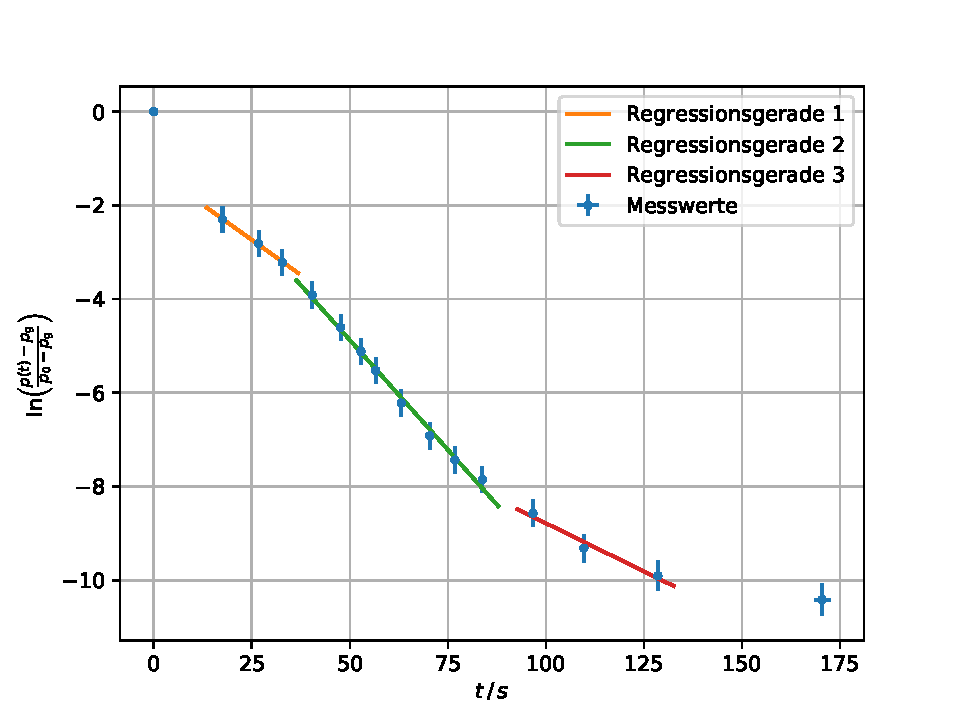
\includegraphics[width=0.85\textwidth]{../Messdaten/plots/dreh/druckplot_drehschieber.pdf}
  \caption{Plot der in Tabelle \ref{tab: druck_dreh} gelisteten Messwerte. Zusätzlich sind in der Grafik die bestimmten Ausgleichsgeraden zu sehen.}
  \label{fig: druck_dreh}
\end{figure}
\FloatBarrier

Wie in der Abbildung \ref{fig: druck_dreh} zu erkennen gibt es drei lineare Bereiche.
In diesen Bereichen wird and die Messdaten eine Gerade
\begin{equation}
  \label{eq: geradengleichung}
  g(x)=mx+b
\end{equation}
gefittet. Mit Hilfe einer Regressionsrechnung werden die Parameter der einzelnen Geraden bestimmt:
\begin{align}
  \label{eq: regression_dreh_druck_1}
  \begin{aligned}
  \text{Druckbereich 1} &\text{: 100 - 20 mbar}& \\
  m&=\SI{-5.98\pm0.32 e-2}{\per\second} \\
  b&=\num{-1.24 \pm0.08 }
\end{aligned}
\end{align}

\begin{align}
  \label{eq: regression_dreh_druck_2}
  \begin{aligned}
  \text{Druckbereich 2} &\text{: 20 - 0.2 mbar}& \\
  m&=\SI{-9.36\pm0.29 e-2}{\per\second} \\
  b&=\num{-0.19 \pm0.18 }
\end{aligned}
\end{align}

\begin{align}
  \label{eq: regression_dreh_druck_3}
  \begin{aligned}
  \text{Druckbereich 3} &\text{: 0.2 - 0.04 mbar}& \\
  m&=\SI{-4.1\pm0.7 e-2}{\per\second} \\
  b&=\num{-4.7 \pm0.8 }
\end{aligned}
\end{align}

Aus der Steigung und dem Volumen kann dann die Saugleistung ermittlt werden:
\begin{equation}
  \label{eq: saug_druck}
  S\ua{eff}=-mV, \qquad \sigma_{S}=\sqrt{\sigma_{m}^{2} V^{2} + \sigma_{V}^{2} m^{2}}.
\end{equation}
Für die Saugleistung der Dreheschieberpumpe ergigbt sich:
\begin{align}
  \label{eq:dreh_saug_1}
  \begin{aligned}
  \text{Druckbereich 1} &\text{: 100 - 20 mbar}& \\
   S\ua{eff}&=\SI{0.59\pm 0.05}{\litre\per\second}
\end{aligned}
\end{align}

\begin{align}
  \label{eq:dreh_saug_2}
  \begin{aligned}
  \text{Druckbereich 2} &\text{: 20 - 0.2 mbar}& \\
   S\ua{eff}&=\SI{0.92\pm 0.06}{\litre\per\second}
\end{aligned}
\end{align}

\begin{align}
  \label{eq:dreh_saug_3}
  \begin{aligned}
  \text{Druckbereich 3} &\text{: 0.2 - 0.04 mbar}& \\
   S\ua{eff}&=\SI{0.40\pm 0.08}{\litre\per\second}
\end{aligned}
\end{align}

Nach Herstellerangabe besitzt die Drehschieberpumpe ein Saugvermögen von $S_0=\SI{1.1}{\litre\per\second}$.
Aus dem experiementell bestimmten Saugvermögen und den Herstellerangabe kann ein Leitwert $L$ errechnet werden.
Gegeben ist der Leitwert durch
\begin{equation*}
  L=\frac{S\ua{eff} S_0}{S_0-S\ua{eff}}, \qquad \sigma_L=\sqrt{ \sigma_{S\ua{eff}}^{2} \left(\frac{S_{0} S\ua{eff}}{\left(S_{0} - S\ua{eff}\right)^{2}} + \frac{S_{0}}{S_{0} - S\ua{eff}}\right)^{2}}.
\end{equation*}
Somit ist der Leitwert für die verschiedenen Druckbereiche:
\begin{align}
  \label{eq:dreh_leit_1}
  \begin{aligned}
  \text{Druckbereich 1} &\text{: 100 - 20 mbar}& \\
   L&=\SI{1.26\pm 0.21}{\litre\per\second}
\end{aligned}
\end{align}

\begin{align}
  \label{eq:dreh_leit_2}
  \begin{aligned}
  \text{Druckbereich 2} &\text{: 20 - 0.2 mbar}& \\
   L&=\SI{5.6\pm 2.2}{\litre\per\second}
\end{aligned}
\end{align}

\begin{align}
  \label{eq:dreh_leit_3}
  \begin{aligned}
  \text{Druckbereich 3} &\text{: 0.2 - 0.04 mbar}& \\
   L&=\SI{0.64\pm 0.19}{\litre\per\second}
\end{aligned}
\end{align}

\subsection{Auswertung Leckkratenmethode}

Die Aufgenommenen Messwerte sind in den Tabellen \ref{tab: leck_dreh_leck_0.1.pdf} - \ref{tab: leck_dreh_leck_1.0.pdf} aufgelistet.
\begin{table} 
\centering 
\caption{Gemessene Drücke bei der Leckkratenmethode für die Drehschieberpumpe mit $p_{\mathrm{g}}=\SI{0.1\pm0.02}{\milli\bar}$. Messung bei Raumtemperatur.} 
\label{tab: leck_dreh_leck_0.1.pdf} 
\begin{tabular}{S[table-format=1.2]@{${}\pm{}$} S[table-format=1.2] S S S S[table-format=1.2]@{${}\pm{}$} S[table-format=1.2] } 
\toprule  
\multicolumn{2}{c}{$p \:/\: \si{ \milli\bar}$} & {$t_1 / \si{ \second}$} & {$t_2 / \si{ \second}$} & {$t_3 / \si{ \second}$} & \multicolumn{2}{c}{$\overline{t} \:/\: \si{ \second}$} \\ 
\midrule  
0.10 & 0.02 & 0.0 & 0.0 & 0.0 & 0.00 & 0.00\\ 
0.20 & 0.04 & 10.3 & 10.8 & 11.5 & 10.87 & 0.34\\ 
0.40 & 0.08 & 50.4 & 50.9 & 51.9 & 51.04 & 0.42\\ 
0.60 & 0.12 & 105.3 & 104.5 & 107.3 & 105.74 & 0.83\\ 
0.80 & 0.16 & 155.4 & 156.3 & 156.7 & 156.12 & 0.36\\ 
1.00 & 0.20 & 199.9 & 199.9 & 201.0 & 200.28 & 0.37\\ 
\bottomrule 
\end{tabular} 
\end{table}

\begin{table} 
\centering 
\caption{Gemessene Drücke bei der Leckkratenmethode für die Drehschieberpumpe mit $p_{\mathrm{g}}=\SI{0.4\pm0.08}{\milli\bar}$. Messung bei Raumtemperatur.} 
\label{tab: leck_dreh_leck_0.4.pdf} 
\begin{tabular}{S[table-format=1.2]@{${}\pm{}$} S[table-format=1.2] S S S S[table-format=1.2]@{${}\pm{}$} S[table-format=1.2] } 
\toprule  
\multicolumn{2}{c}{$p \:/\: \si{ \milli\bar}$} & {$t_1 / \si{ \second}$} & {$t_2 / \si{ \second}$} & {$t_3 / \si{ \second}$} & \multicolumn{2}{c}{$\overline{t} \:/\: \si{ \second}$} \\ 
\midrule  
0.40 & 0.08 & 0.0 & 0.0 & 0.0 & 0.00 & 0.00\\ 
0.60 & 0.12 & 7.5 & 8.1 & 7.5 & 7.69 & 0.21\\ 
0.80 & 0.16 & 15.7 & 16.7 & 15.7 & 16.07 & 0.33\\ 
1.00 & 0.20 & 23.8 & 23.4 & 23.8 & 23.64 & 0.14\\ 
2.00 & 0.40 & 58.9 & 58.7 & 58.9 & 58.87 & 0.07\\ 
4.00 & 0.80 & 117.1 & 118.4 & 117.1 & 117.54 & 0.44\\ 
\bottomrule 
\end{tabular} 
\end{table}

\begin{table} 
\centering 
\caption{Gemessene Drücke bei der Leckkratenmethode für die Drehschieberpumpe mit $p_{\mathrm{g}}=\SI{0.8\pm0.16}{\milli\bar}$. Messung bei Raumtemperatur.} 
\label{tab: leck_dreh_leck_0.8.pdf} 
\begin{tabular}{S[table-format=1.2]@{${}\pm{}$} S[table-format=1.2] S S S S[table-format=1.2]@{${}\pm{}$} S[table-format=1.2] } 
\toprule  
\multicolumn{2}{c}{$p \:/\: \si{ \milli\bar}$} & {$t_1 / \si{ \second}$} & {$t_2 / \si{ \second}$} & {$t_3 / \si{ \second}$} & \multicolumn{2}{c}{$\overline{t} \:/\: \si{ \second}$} \\ 
\midrule  
0.80 & 0.16 & 0.0 & 0.0 & 0.0 & 0.00 & 0.00\\ 
1.00 & 0.20 & 2.9 & 2.9 & 2.9 & 2.87 & 0.02\\ 
2.00 & 0.40 & 15.5 & 15.8 & 15.5 & 15.62 & 0.09\\ 
4.00 & 0.80 & 37.9 & 38.0 & 37.9 & 37.95 & 0.03\\ 
6.00 & 1.20 & 57.8 & 57.8 & 57.8 & 57.78 & 0.01\\ 
8.00 & 1.60 & 80.3 & 80.5 & 80.3 & 80.35 & 0.07\\ 
\bottomrule 
\end{tabular} 
\end{table}

\begin{table} 
\centering 
\caption{Gemessene Drücke bei der Leckkratenmethode für die Drehschieberpumpe mit $p_{\mathrm{g}}=\SI{1.0\pm0.20}{\milli\bar}$. Messung bei Raumtemperatur.} 
\label{tab: leck_dreh_leck_1.0.pdf} 
\begin{tabular}{S[table-format=1.2]@{${}\pm{}$} S[table-format=1.2] S S S S[table-format=1.2]@{${}\pm{}$} S[table-format=1.2] } 
\toprule  
\multicolumn{2}{c}{$p \:/\: \si{ \milli\bar}$} & {$t_1 / \si{ \second}$} & {$t_2 / \si{ \second}$} & {$t_3 / \si{ \second}$} & \multicolumn{2}{c}{$\overline{t} \:/\: \si{ \second}$} \\ 
\midrule  
1.00 & 0.20 & 0.0 & 0.0 & 0.0 & 0.00 & 0.00\\ 
2.00 & 0.40 & 10.3 & 10.1 & 10.3 & 10.26 & 0.06\\ 
4.00 & 0.80 & 28.1 & 28.3 & 28.1 & 28.20 & 0.05\\ 
6.00 & 1.20 & 44.6 & 44.0 & 44.6 & 44.39 & 0.18\\ 
8.00 & 1.60 & 62.5 & 61.3 & 62.5 & 62.11 & 0.40\\ 
10.00 & 2.00 & 79.3 & 80.0 & 79.3 & 79.51 & 0.24\\ 
\bottomrule 
\end{tabular} 
\end{table}


Die gemittelten Zeiten wurden mit \eqref{eq: mittel} und \eqref{eq: standartabweichung} bestimmt
Eine graphische Darstellung der Werte ist in den Abbildung \ref{fig: leck_dreh_1} und \ref{fig: leck_dreh_2} dargestellt.

\begin{figure}
    \centering
    \begin{subfigure}{0.4\textwidth}
        \centering
        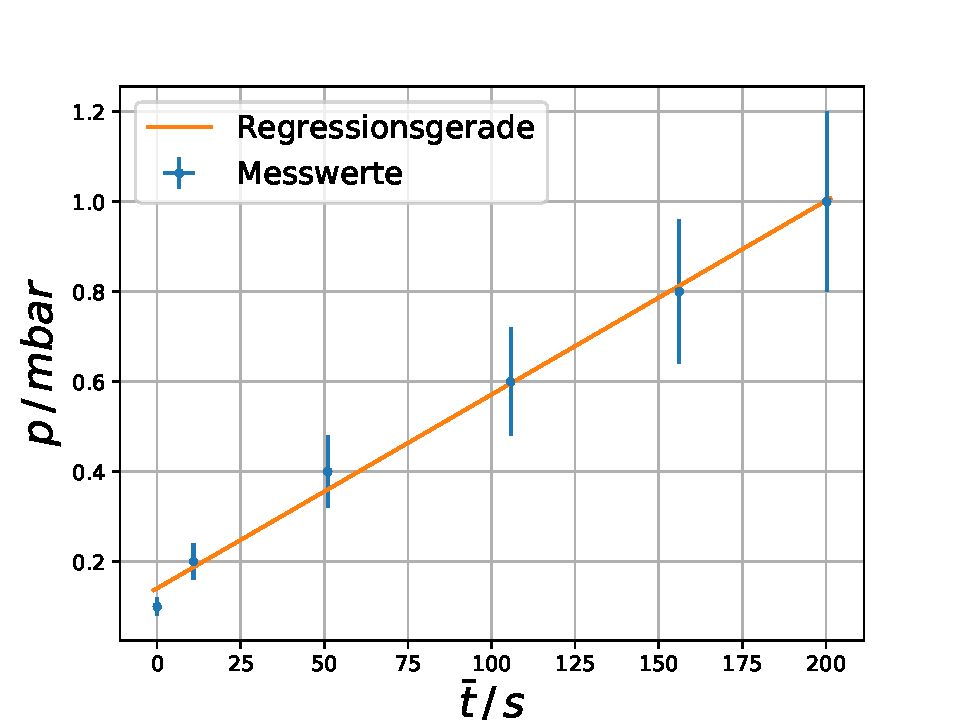
\includegraphics[width=1\textwidth]{../Messdaten/plots/dreh/leckrate_dreh_01.pdf}
        \caption{Grafische Darstellung der Tabelle \ref{tab: leck_dreh_leck_0.1.pdf}. Zusätzlich ist die Ausgleichsgerade zu erkennen.}
        \label{fig: drehs_leck_1}
    \end{subfigure}
    \begin{subfigure}{0.4\textwidth}
        \centering
        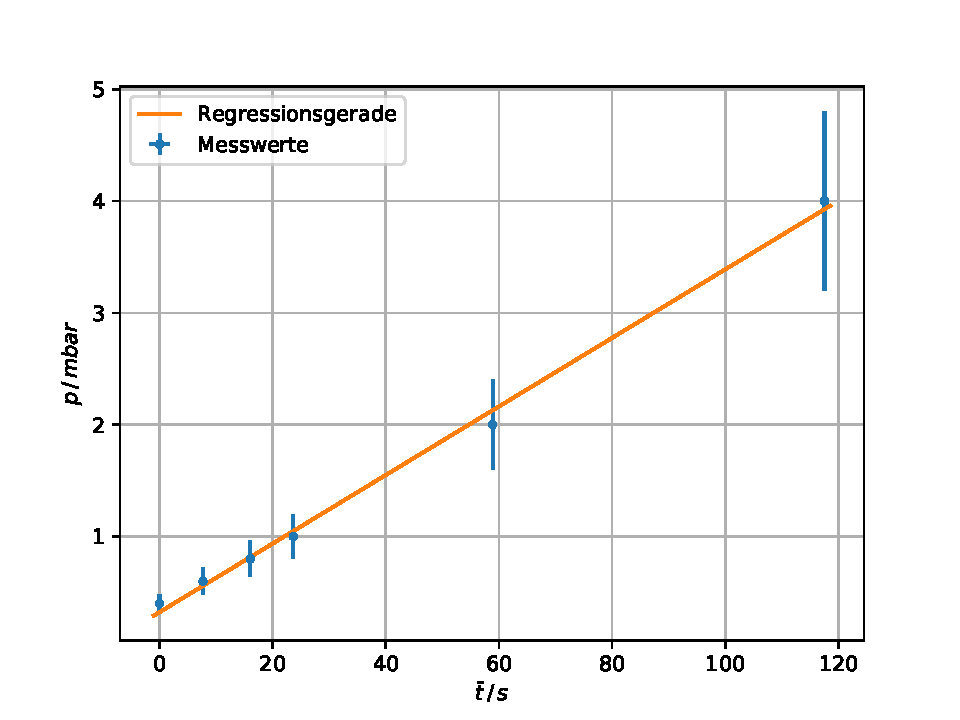
\includegraphics[width=1\textwidth]{../Messdaten/plots/dreh/leckrate_dreh_04.pdf}
        \caption{Grafische Darstellung der Tabelle \ref{tab: leck_dreh_leck_0.4.pdf}. Zusätzlich ist die Ausgleichsgerade zu erkennen.}
    \end{subfigure}
    \caption{Leckratenmessung für die Drehschieberpumpe}
      \label{fig: leck_dreh_1}
\end{figure}

\begin{figure}
    \centering
    \begin{subfigure}{0.4\textwidth}
        \centering
        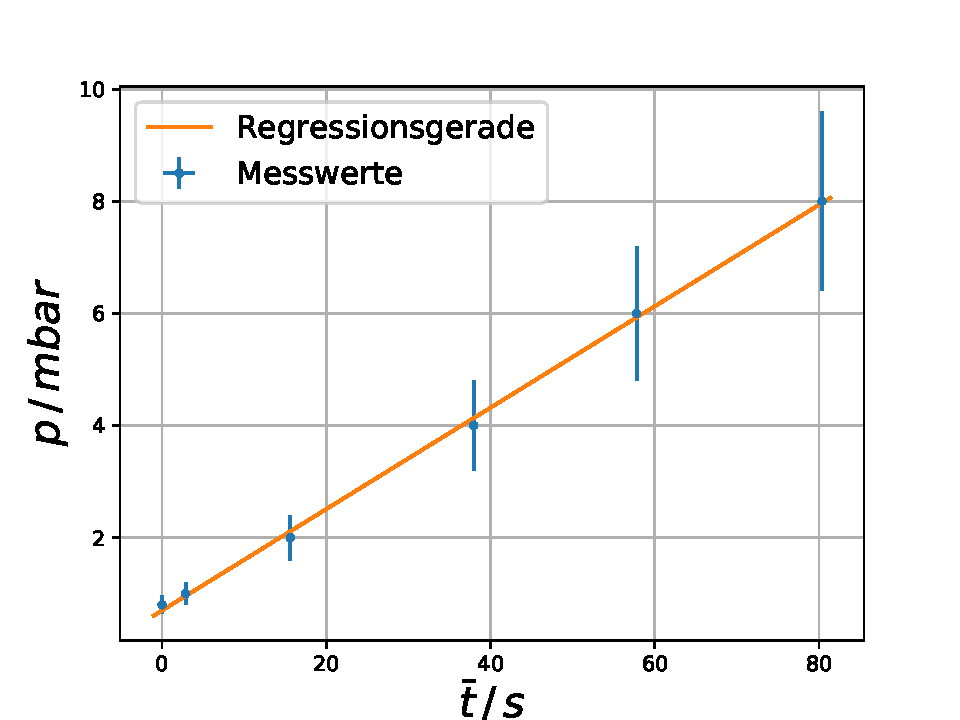
\includegraphics[width=1\textwidth]{../Messdaten/plots/dreh/leckrate_dreh_08.pdf}
        \caption{Grafische Darstellung der Tabelle \ref{tab: leck_dreh_leck_0.8.pdf}. Zusätzlich ist die Ausgleichsgerade zu erkennen.}
        \label{fig: drehs_leck_1}
    \end{subfigure}
    \begin{subfigure}{0.4\textwidth}
        \centering
        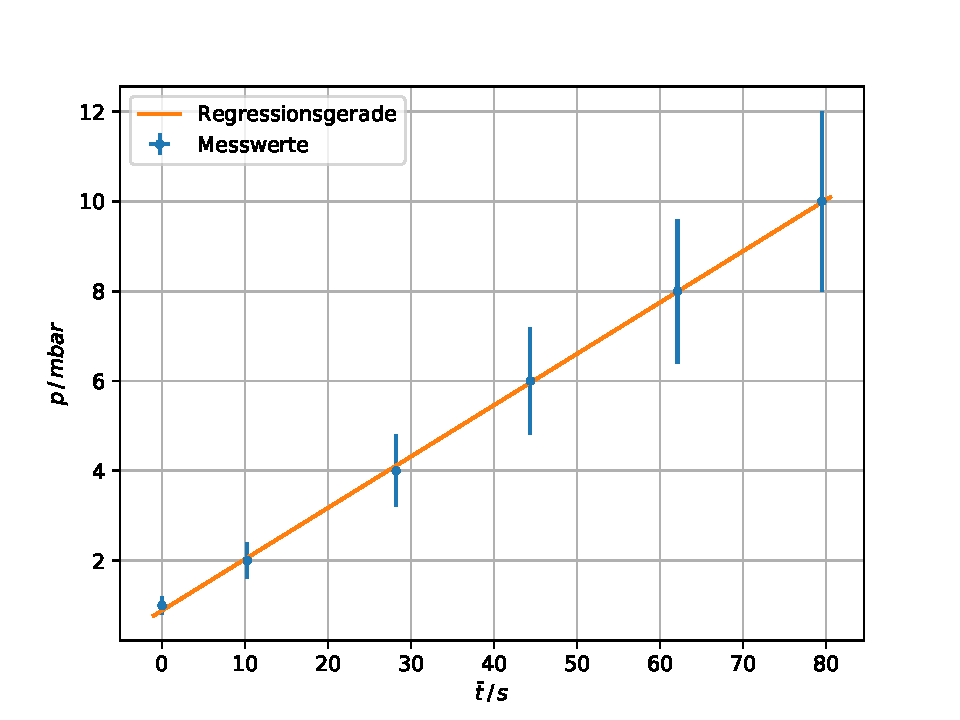
\includegraphics[width=1\textwidth]{../Messdaten/plots/dreh/leckrate_dreh_10.pdf}
        \caption{Grafische Darstellung der Tabelle \ref{tab: leck_dreh_leck_1.0.pdf}. Zusätzlich ist die Ausgleichsgerade zu erkennen.}
    \end{subfigure}
    \caption{Leckratenmessung für die Drehschieberpumpe}
      \label{fig: leck_dreh_2}
\end{figure}
Mittels Regressionsrechnunge wurden die in den Abbildung eingezeichneten Ausgleichsgeraden ermittelt.
Dabei werden die Messwerte an eine Gerade (vgl. \eqref{eq: geradengleichung}) gefittet.
Aus der Regressionsrechnung ergeben sich die folgenden Parameter

\begin{align*}
  \text{Gleichgewichtsdruck:} &\, p_g=\SI{0.1}{\milli\bar} \\
  m&= \SI{4.31\pm 0.17 e-3 }{\milli\bar\per\second}\\
  b&=\SI{14.1\pm1.9 e-2}{\milli\bar}\\
  \\
  \text{Gleichgewichtsdruck:} &\, p_g=\SI{0.4}{\milli\bar} \\
  m&= \SI{3.07\pm 0.09 e-2 }{\milli\bar\per\second}\\
  b&=\SI{32\pm5 e-2}{\milli\bar}\\
  \\
  \text{Gleichgewichtsdruck:} &\, p_g=\SI{0.8}{\milli\bar}\\
  m&= \SI{9.05\pm 0.15 e-2 }{\milli\bar\per\second}\\
  b&=\SI{70\pm7 e-2}{\milli\bar}\\
  \\
  \text{Gleichgewichtsdruck:} &\, p_g=\SI{1}{\milli\bar}\\
  m&= \SI{11.43\pm 0.13 e-2 }{\milli\bar\per\second}\\
  b&=\SI{89\pm 6 e-2}{\milli\bar}
\end{align*}

Das Saugvermögen kann aus Gleichung
\begin{equation}
  \label{eq:saug_leck}
  S=\frac{Vm}{p_g}, \qquad \sigma_{S}=\sqrt{\frac{V^{2} \sigma_{m}^{2}}{p_{g}^{2}} + \frac{V^{2} \sigma_{p_{g}}^{2}}{p_{g}^{4}} m^{2} + \frac{\sigma_{V}^{2} m^{2}}{p_{g}^{2}}}
\end{equation}
bestimmt werden.
\begin{align*}
  \text{Gleichgewichtsdruck:} &\, p_g=\SI{0.1}{\milli\bar} \\
  S&=\SI{0.42\pm 0.09}{\litre\per\second}
  \\
  \text{Gleichgewichtsdruck:} &\, p_g=\SI{0.4}{\milli\bar} \\
  S&=\SI{0.75\pm 0.16}{\litre\per\second}
  \\
  \text{Gleichgewichtsdruck:} &\, p_g=\SI{0.8}{\milli\bar}\\
  S&=\SI{1.11\pm 0.23}{\litre\per\second}
  \\
  \text{Gleichgewichtsdruck:} &\, p_g=\SI{1}{\milli\bar}\\
  S&=\SI{1.12\pm 0.23}{\litre\per\second}
\end{align*}

\textbf{Vergleichs Plot fehlt noch}
